\documentclass[aspectratio=169,11pt,xcolor=table]{beamer}
\usepackage{tikz}
\usetikzlibrary{arrows.meta,positioning,shapes.geometric,fit,calc,backgrounds}
\usepackage{pgfgantt}
\usepackage{amsmath,amssymb}
\usepackage{booktabs}
\usepackage{graphicx}
\usepackage{appendixnumberbeamer}
\hypersetup{hidelinks}
\definecolor{utadblue}{RGB}{0,46,93}
\definecolor{accent}{RGB}{200,16,46}
\definecolor{accentlight}{RGB}{230,210,215}
\definecolor{sevmed}{RGB}{255,230,230}
\definecolor{sevlow}{RGB}{235,235,235}
\IfFileExists{beamerthememetropolis.sty}{%
  \usetheme[progressbar=frametitle,numbering=fraction,sectionpage=progressbar,block=fill]{metropolis}%
}{%
  \usetheme{default}%
  \setbeamerfont{frametitle}{series=\bfseries}%
}
\setbeamercolor{progress bar}{fg=accent}
\setbeamercolor{frametitle}{bg=utadblue}
\setbeamercolor{alerted text}{fg=accent}
\setbeamercolor{section title}{fg=utadblue}
\setbeamertemplate{navigation symbols}{}

\title{Clinically-Deployable 3D Vascular and Organ Segmentation from CT}
\subtitle{PhD Thesis Plan Defense --- Doutoramento em Informática}
\author{Alexandre Tolstenko Nogueira}
\institute{{\small Universidade de Trás-os-Montes e Alto Douro} \\ {\scriptsize Orientador: Vitor Manuel de Jesus Filipe \\ Coorientador: Nuno Miguel Fonseca Ferreira}}
\date{17 July 2026}
\begin{document}

\begin{frame}[plain]
\titlepage
\begin{tikzpicture}[remember picture, overlay]
  \node[anchor=south east, xshift=-0.5cm, yshift=0.4cm] at (current page.south east) {
    
\includegraphics[height=0.8cm]{figures/utad_azul.png}
  };
\end{tikzpicture}
\end{frame}

\begin{frame}{Outline}
\tableofcontents
\end{frame}

\section{Motivation}
\begin{frame}{Clinical motivation}
\footnotesize
Minimally invasive abdominal surgery depends critically on patient-specific 3D anatomical understanding.
\vspace{0.4cm}
\begin{columns}[T]
\begin{column}{0.48\linewidth}
\begin{block}{Surgical Outcomes}
\vspace{0.1cm}
3D preoperative planning reduces positive surgical margins in partial nephrectomy by \alert{\textbf{23--47\%}} compared to standard imaging.\footnote{\scriptsize Porpiglia et al., \emph{BJU Int.} 121(4):574--581, 2018.}
\vspace{0.2cm}
\end{block}
\end{column}
\begin{column}{0.48\linewidth}
\begin{block}{The Adoption Barrier}
\vspace{0.1cm}
A survey of $N=387$ surgeons shows that \alert{\textbf{68\,\%}} cite ``time-intensive preparation'' as the primary barrier to clinical adoption.\footnote{\scriptsize Simpfend\"orfer et al., \emph{J.~Robotic Surg.} 10(4):321--329, 2016.}
\vspace{0.2cm}
\end{block}
\end{column}
\end{columns}
\end{frame}

\begin{frame}{Context: The DocDo clinical pipeline}
\footnotesize
\begin{columns}[c]
\begin{column}{0.5\linewidth}
  \centering
  \fcolorbox{utadblue!20}{white}{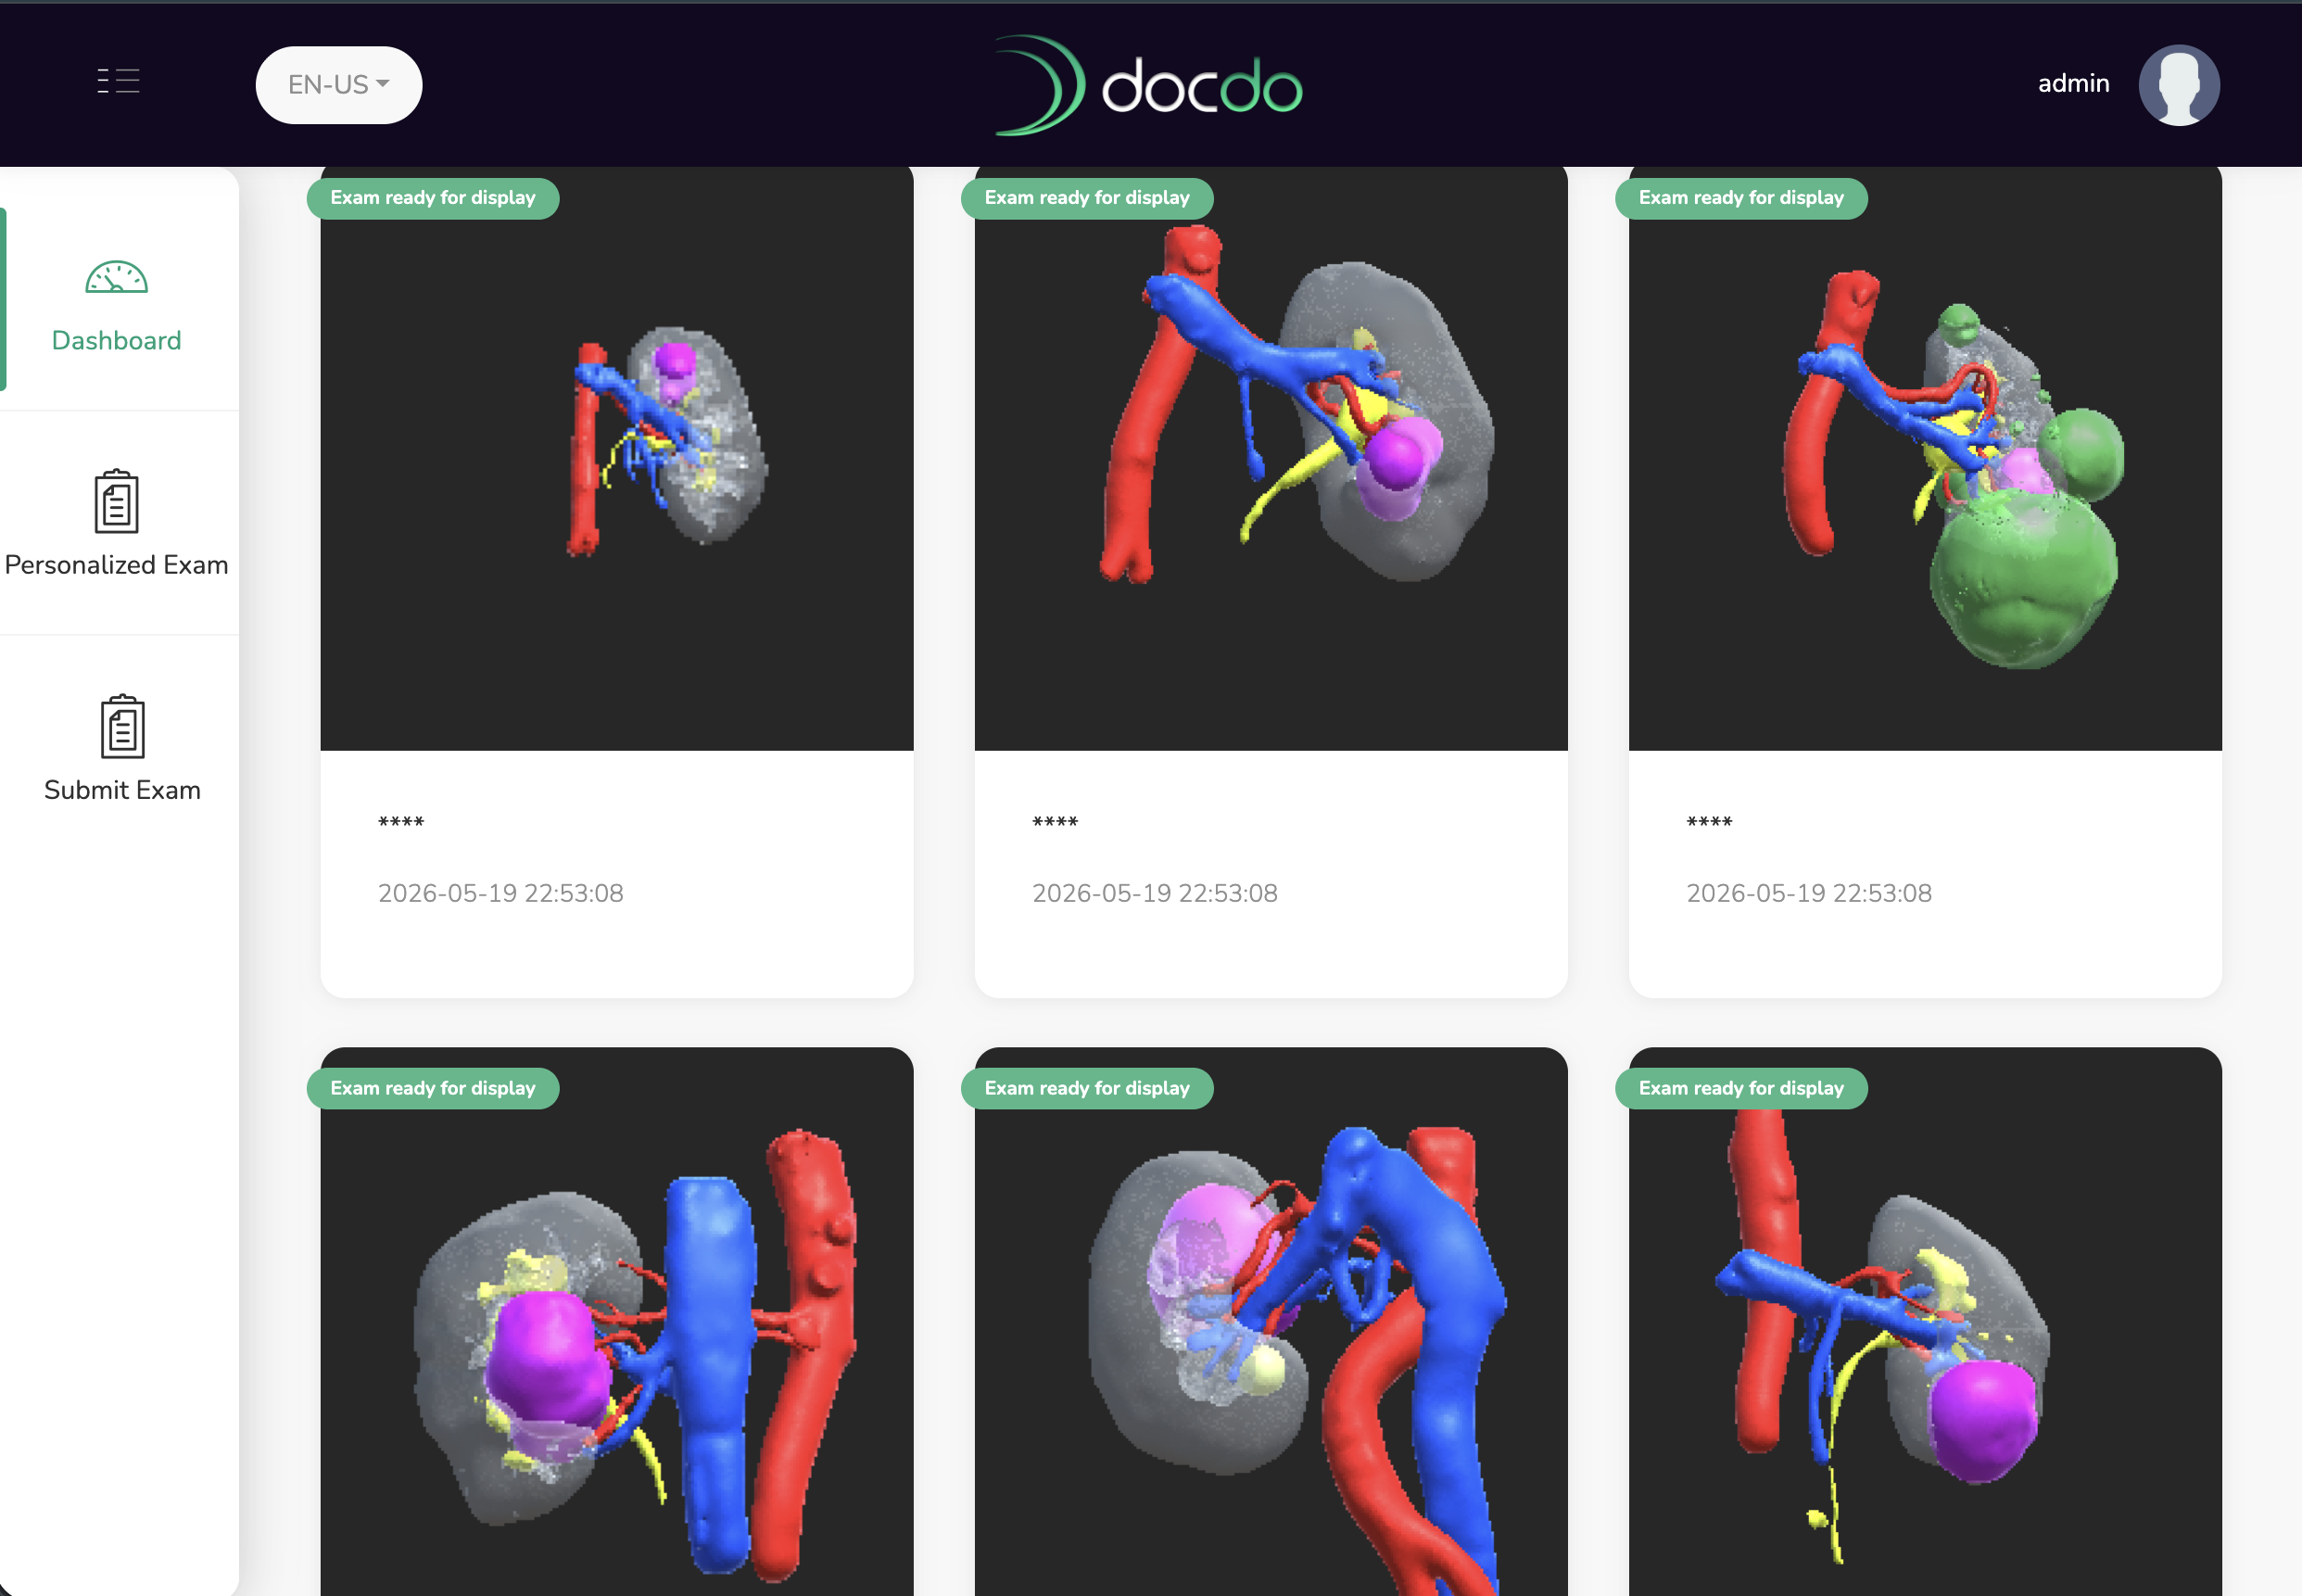
\includegraphics[width=0.95\linewidth]{figures/backoffice.png}}
  \vspace{0.15cm}
  \scriptsize\color{gray} Clinical prototype tested on 1,000+ cases over 10 years
\end{column}
\begin{column}{0.46\linewidth}
  \begin{block}{Surgeon Requirements}
    \begin{itemize}
    \setlength\itemsep{5pt}
    \item \textbf{Controllability:} Fast interactive edits ($\le 2$s)
    \item \textbf{Auditability:} Clear voxel-level path costs
    \item \textbf{Robustness:} Works across scanners \& protocols
    \item \textbf{Sub-voxel Accuracy:} Crucial for tumor-vessel margins
    \end{itemize}
  \end{block}
\end{column}
\end{columns}
\end{frame}

\begin{frame}{A saturated state of the art}
\footnotesize
\begin{columns}[c]
\begin{column}{0.52\linewidth}
  \centering
  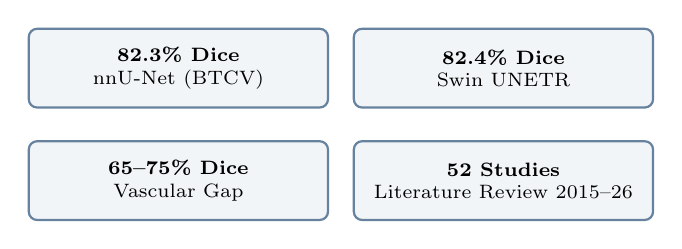
\begin{tikzpicture}[
    node distance=0.4cm and 0.3cm,
    stat/.style={rectangle, draw=utadblue!60, thick, rounded corners=3pt, minimum width=3.8cm, minimum height=1.0cm, align=center, font=\scriptsize, fill=utadblue!5}
  ]
    \node[stat] (d1) {\textbf{82.3\% Dice} \\ nnU-Net (BTCV)};
    \node[stat, right=of d1] (d2) {\textbf{82.4\% Dice} \\ Swin UNETR};
    \node[stat, below=of d1] (d3) {\textbf{65--75\% Dice} \\ Vascular Gap};
    \node[stat, right=of d3] (d4) {\textbf{52 Studies} \\ Literature Review 2015--26};
  \end{tikzpicture}
\end{column}
\begin{column}{0.44\linewidth}
  \begin{block}{State of the Art Ceilings \& Gaps}
    \begin{itemize}
    \setlength\itemsep{4pt}
    \item \textbf{Parenchyma Ceiling:} No significant difference between CNN and Transformer.
    \item \textbf{Vascular Deficit:} Markedly lower accuracy due to topological complexity.
    \item \textbf{Overlap Bias:} Dice scores fail to measure topological correctness.
    \end{itemize}
  \end{block}
\end{column}
\end{columns}
\vspace{0.15cm}
\vspace{0.1cm}
\end{frame}

\begin{frame}{Deep-learning timeline}
\footnotesize
\begin{columns}[T]
\begin{column}{0.48\linewidth}
\scriptsize
\begin{enumerate}
\setlength\itemsep{0pt}
\setlength\parskip{0pt}
\setlength\parsep{0pt}
\item \textbf{U-Net} (Ronneberger, 2015) --- encoder--decoder + skips, 2D
\item \textbf{3D U-Net} (\c{c}i\c{c}ek, 2016) --- volumetric 3D conv
\item \textbf{V-Net} (Milletari, 2016) --- Dice-loss training
\item \textbf{nnU-Net} (Isensee, 2021) --- self-configuring; \alert{82.3\% Dice} on BTCV (multi-organ benchmark)
\item \textbf{UNETR / Swin UNETR} (Hatamizadeh, 2022) --- ViT / shifted-window; Swin \alert{82.4\%} BTCV
\item \textbf{TotalSegmentator} (Wasserthal, 2023) --- 117 structures off-the-shelf
\item \textbf{MedSAM / SAM-Med3D} (Ma / Wang, 2024) --- prompt-driven foundation models
\end{enumerate}
\end{column}
\begin{column}{0.48\linewidth}
\begin{block}{Saturated SOTA --- Review Findings}
\scriptsize
\begin{itemize}
\setlength\itemsep{4pt}
\item CNNs dominate literature: \alert{\textbf{98.1\,\%}} of 52 studies.
\item 3D U-Net variants in \alert{\textbf{82.7\,\%}} of studies.
\item Parenchyma Dice plateau: \alert{$\approx 82\%$} regardless of paradigm (CNN vs Transformer).
\item Confidence intervals overlap; no significant difference between nnU-Net and Swin UNETR.
\item Foundation models: remarkable zero-shot coverage; underperform on vessels and surgeon-grade margins.
\end{itemize}
\end{block}
\vspace{0.15cm}
\scriptsize\color{gray}Sources: 52-study SLR (2015--Jan.~2026).
\end{column}
\end{columns}
\end{frame}

\begin{frame}{Preliminary work}
\scriptsize
\begin{columns}[T]
\begin{column}{0.48\linewidth}
\begin{block}{Legacy Desktop Application}
  \begin{itemize}
  \setlength\itemsep{2pt}
  \item \textbf{Segmentation:} 3D Slicer + Python
  \item \textbf{Post-processing:} MeshLab
  \item \textbf{Visualization:} Unity-based desktop client
  \item \textbf{Infrastructure:} PHP web portal
  \end{itemize}
\end{block}
\end{column}
\begin{column}{0.48\linewidth}
\begin{block}{Proposed Web Prototype}
  \begin{itemize}
  \setlength\itemsep{2pt}
  \item \textbf{Web UI:} Next.js prototype webpage
  \item \textbf{Core Editor:} C++/WASM (WebAssembly) + GDCM (DICOM library)
  \item \textbf{UI \& Windowing:} RmlUi + SDL3 (Simple DirectMedia Layer)
  \item \textbf{Graphics API:} WebGPU (Dawn)
  \item \textbf{Execution:} Browser-based C++/WASM runs
  \end{itemize}
\end{block}
\end{column}
\end{columns}

\vspace{0.15cm}
\begin{columns}[T]
\begin{column}{0.7\linewidth}
  \textbf{Development Status:} \\
  \textcolor{accent}{$\checkmark$} Web framework,
  \textcolor{accent}{$\checkmark$} Secure data transfer,
  \textcolor{accent}{$\checkmark$} Volume rendering engine \\
  \textcolor{gray}{$\times$} DICOMdir parser \quad
  \textcolor{gray}{$\times$} 3D Editor body \quad
  \textcolor{gray}{$\times$} Clinical site validation
\end{column}
\begin{column}{0.31\linewidth}
  \raggedleft
  \color{gray}\tiny
  Contacts: Hosp.\ São Marcos; UDI Teresina; 
\end{column}
\end{columns}
\end{frame}

\section{The deterministic pipeline}

\begin{frame}{Seeded Image Foresting Transform (IFT)}
\footnotesize
\textit{Core intuition: Each voxel is labelled by the seed whose cheapest path reaches it.}

\vspace{0.2cm}
\begin{columns}[T]
\begin{column}{0.48\linewidth}
  \begin{block}{1. The Theoretical Foundation (Falc\~ao 2004)}
    \begin{itemize}
    \setlength\itemsep{4pt}
    \item \textbf{Search Model:} Optimum-path forest; grows one labelled tree per seed.
    \item \textbf{Path Cost:} \emph{Bottleneck} --- evaluates the worst edge on the best path.
    \item \textbf{The Clinical Barrier:} Unifies region-growing algorithms perfectly, but has \alert{no built-in latency budget} for real-time surgical editing.
    \end{itemize}
  \end{block}
\end{column}
\begin{column}{0.48\linewidth}
  \begin{block}{2. The DocDo Clinical Adaptation}
    \begin{itemize}
    \setlength\itemsep{4pt}
    \item \textbf{Search Model:} Multi-source Dijkstra on a priority queue. It feels like an controlled watershed.
    \item \textbf{Path Cost:} \emph{Additive} --- sum of intensity differences $|I(u)-I(v)|$ over edges.
    \item \textbf{The Solution:} Engineered \alert{budgets} (cost caps), \alert{thresholds} (seed-stats), and \alert{iteration ceilings}.
    \item \textbf{Result:} A deterministic, auditable, and \textbf{surgeon-controllable} tool.
    \end{itemize}
  \end{block}
\end{column}
\end{columns}
\end{frame}

\begin{frame}{Seeded IFT — flow diagram}
\footnotesize
\begin{center}
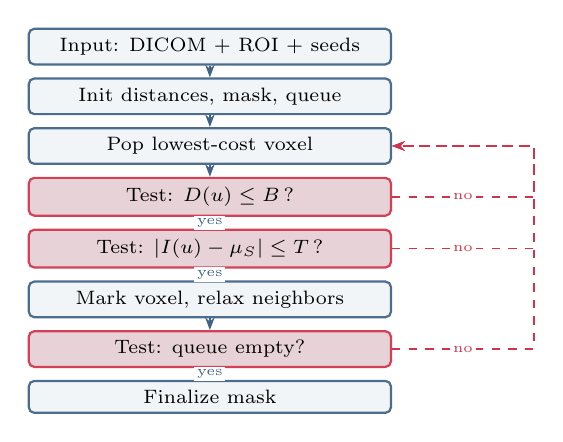
\begin{tikzpicture}[
  node distance=0.15cm and 0.4cm,
  proc/.style={rectangle, draw=utadblue!70, thick, rounded corners=2pt,
               minimum width=4.6cm, minimum height=0.4cm,
               align=center, font=\scriptsize, fill=utadblue!5},
  dec/.style={rectangle, draw=accent!80, thick, rounded corners=2pt,
              minimum width=4.6cm, minimum height=0.4cm,
              align=center, font=\scriptsize, fill=accentlight},
  yes/.style={-{Stealth[length=1.6mm]}, semithick, utadblue!75},
  no/.style={-{Stealth[length=1.6mm]}, semithick, accent!85, dashed},
  lbl/.style={font=\tiny, midway, fill=white, inner sep=1pt}
]
\node[proc]                    (start)  {Input: DICOM + ROI + seeds};
\node[proc, below=of start]    (init)   {Init distances, mask, queue};
\node[proc, below=of init]     (pop)    {Pop lowest-cost voxel};
\node[dec,  below=of pop]      (budget) {Test: $D(u) \le B$\,?};
\node[dec,  below=of budget]   (thr)    {Test: $|I(u)-\mu_S| \le T$\,?};
\node[proc, below=of thr]      (mark)   {Mark voxel, relax neighbors};
\node[dec,  below=of mark]     (endq)   {Test: queue empty?};
\node[proc, below=of endq]     (Done)   {Finalize mask};

\draw[yes] (start)  -- (init);
\draw[yes] (init)   -- (pop);
\draw[yes] (pop)    -- (budget);
\draw[yes] (budget) -- node[lbl]{yes} (thr);
\draw[yes] (thr)    -- node[lbl]{yes} (mark);
\draw[yes] (mark)   -- (endq);
\draw[yes] (endq)   -- node[lbl]{yes} (Done);

\coordinate (rail) at ($(pop.east)+(1.8,0)$);
\draw[no] (budget.east) -- node[lbl]{no} (budget.east -| rail) |- (pop.east);
\draw[no] (thr.east)    -- node[lbl]{no} (thr.east    -| rail) |- (pop.east);
\draw[no] (endq.east)   -- node[lbl]{no} (endq.east   -| rail) |- (pop.east);
\end{tikzpicture}
\end{center}
\vspace{0.05cm}
{\scriptsize\color{gray} $D(u)$ = accumulated path cost; $B$ = budget; $I(u)$ = voxel intensity; $\mu_S$ = mean seed intensity; $T$ = threshold. ``Relax'' = Dijkstra-style neighbor update. \textcolor{accent}{$\blacksquare$}~decision, \textcolor{utadblue}{$\blacksquare$}~process.}
\end{frame}

\begin{frame}{Orthogonal Vessel Tracker (OVT)}
\footnotesize
\begin{columns}[T]
\begin{column}{0.54\linewidth}
  \begin{block}{Iterative Ridge Tracking Steps}
    \begin{enumerate}
    \setlength\itemsep{4pt}
    \item Compute Hessian in orthogonal plane to propagation
    \item Dominant eigenvector gives orientation \& radius
    \item Fit a Gaussian cross-section model
    \item Advance seed along the ridge
    \end{enumerate}
  \end{block}
\end{column}
\begin{column}{0.42\linewidth}
  \begin{block}{Surgeon-Friendly Design}
    \begin{itemize}
    \setlength\itemsep{4pt}
    \item Produces geometrically explicit centerlines.
    \item Local radius estimation at every point.
    \item Every tracker step is inspectable and auditable in 3D space.
    \end{itemize}
  \end{block}
\end{column}
\end{columns}
\vspace{0.15cm}
{\scriptsize\color{gray} Terms: Hessian = second-derivative matrix capturing local curvature; eigenvector = direction of maximum ridge response; Gaussian = bell-shaped cross-section model; centerline = vessel midline.}
\vspace{0.1cm}
\end{frame}

\begin{frame}{Failure modes}
\footnotesize
\begin{columns}[T]
\begin{column}{0.48\linewidth}
  \begin{block}{Bifurcations}
    Single-ridge model breaks at splits. Eigenstructure of Hessian becomes ambiguous, causing tracker to stall or oscillate.
  \end{block}
\end{column}
\begin{column}{0.48\linewidth}
  \begin{block}{Non-circular Cross-sections}
    Renal and portal veins are frequently elliptical or tortuous. Gaussian model fitting diverges, halting centerlines prematurely.
  \end{block}
\end{column}
\end{columns}
\vspace{0.2cm}
\begin{alertblock}{Clinical Impact on my previous work}
Tracker is implemented but excluded from the active clinical workflow; pipeline falls back to Seeded IFT for vessels, losing topological connectivity.
\end{alertblock}
\vspace{0.1cm}
\end{frame}
\begin{frame}{Elliptical vessel cross-section illustration}
\centering
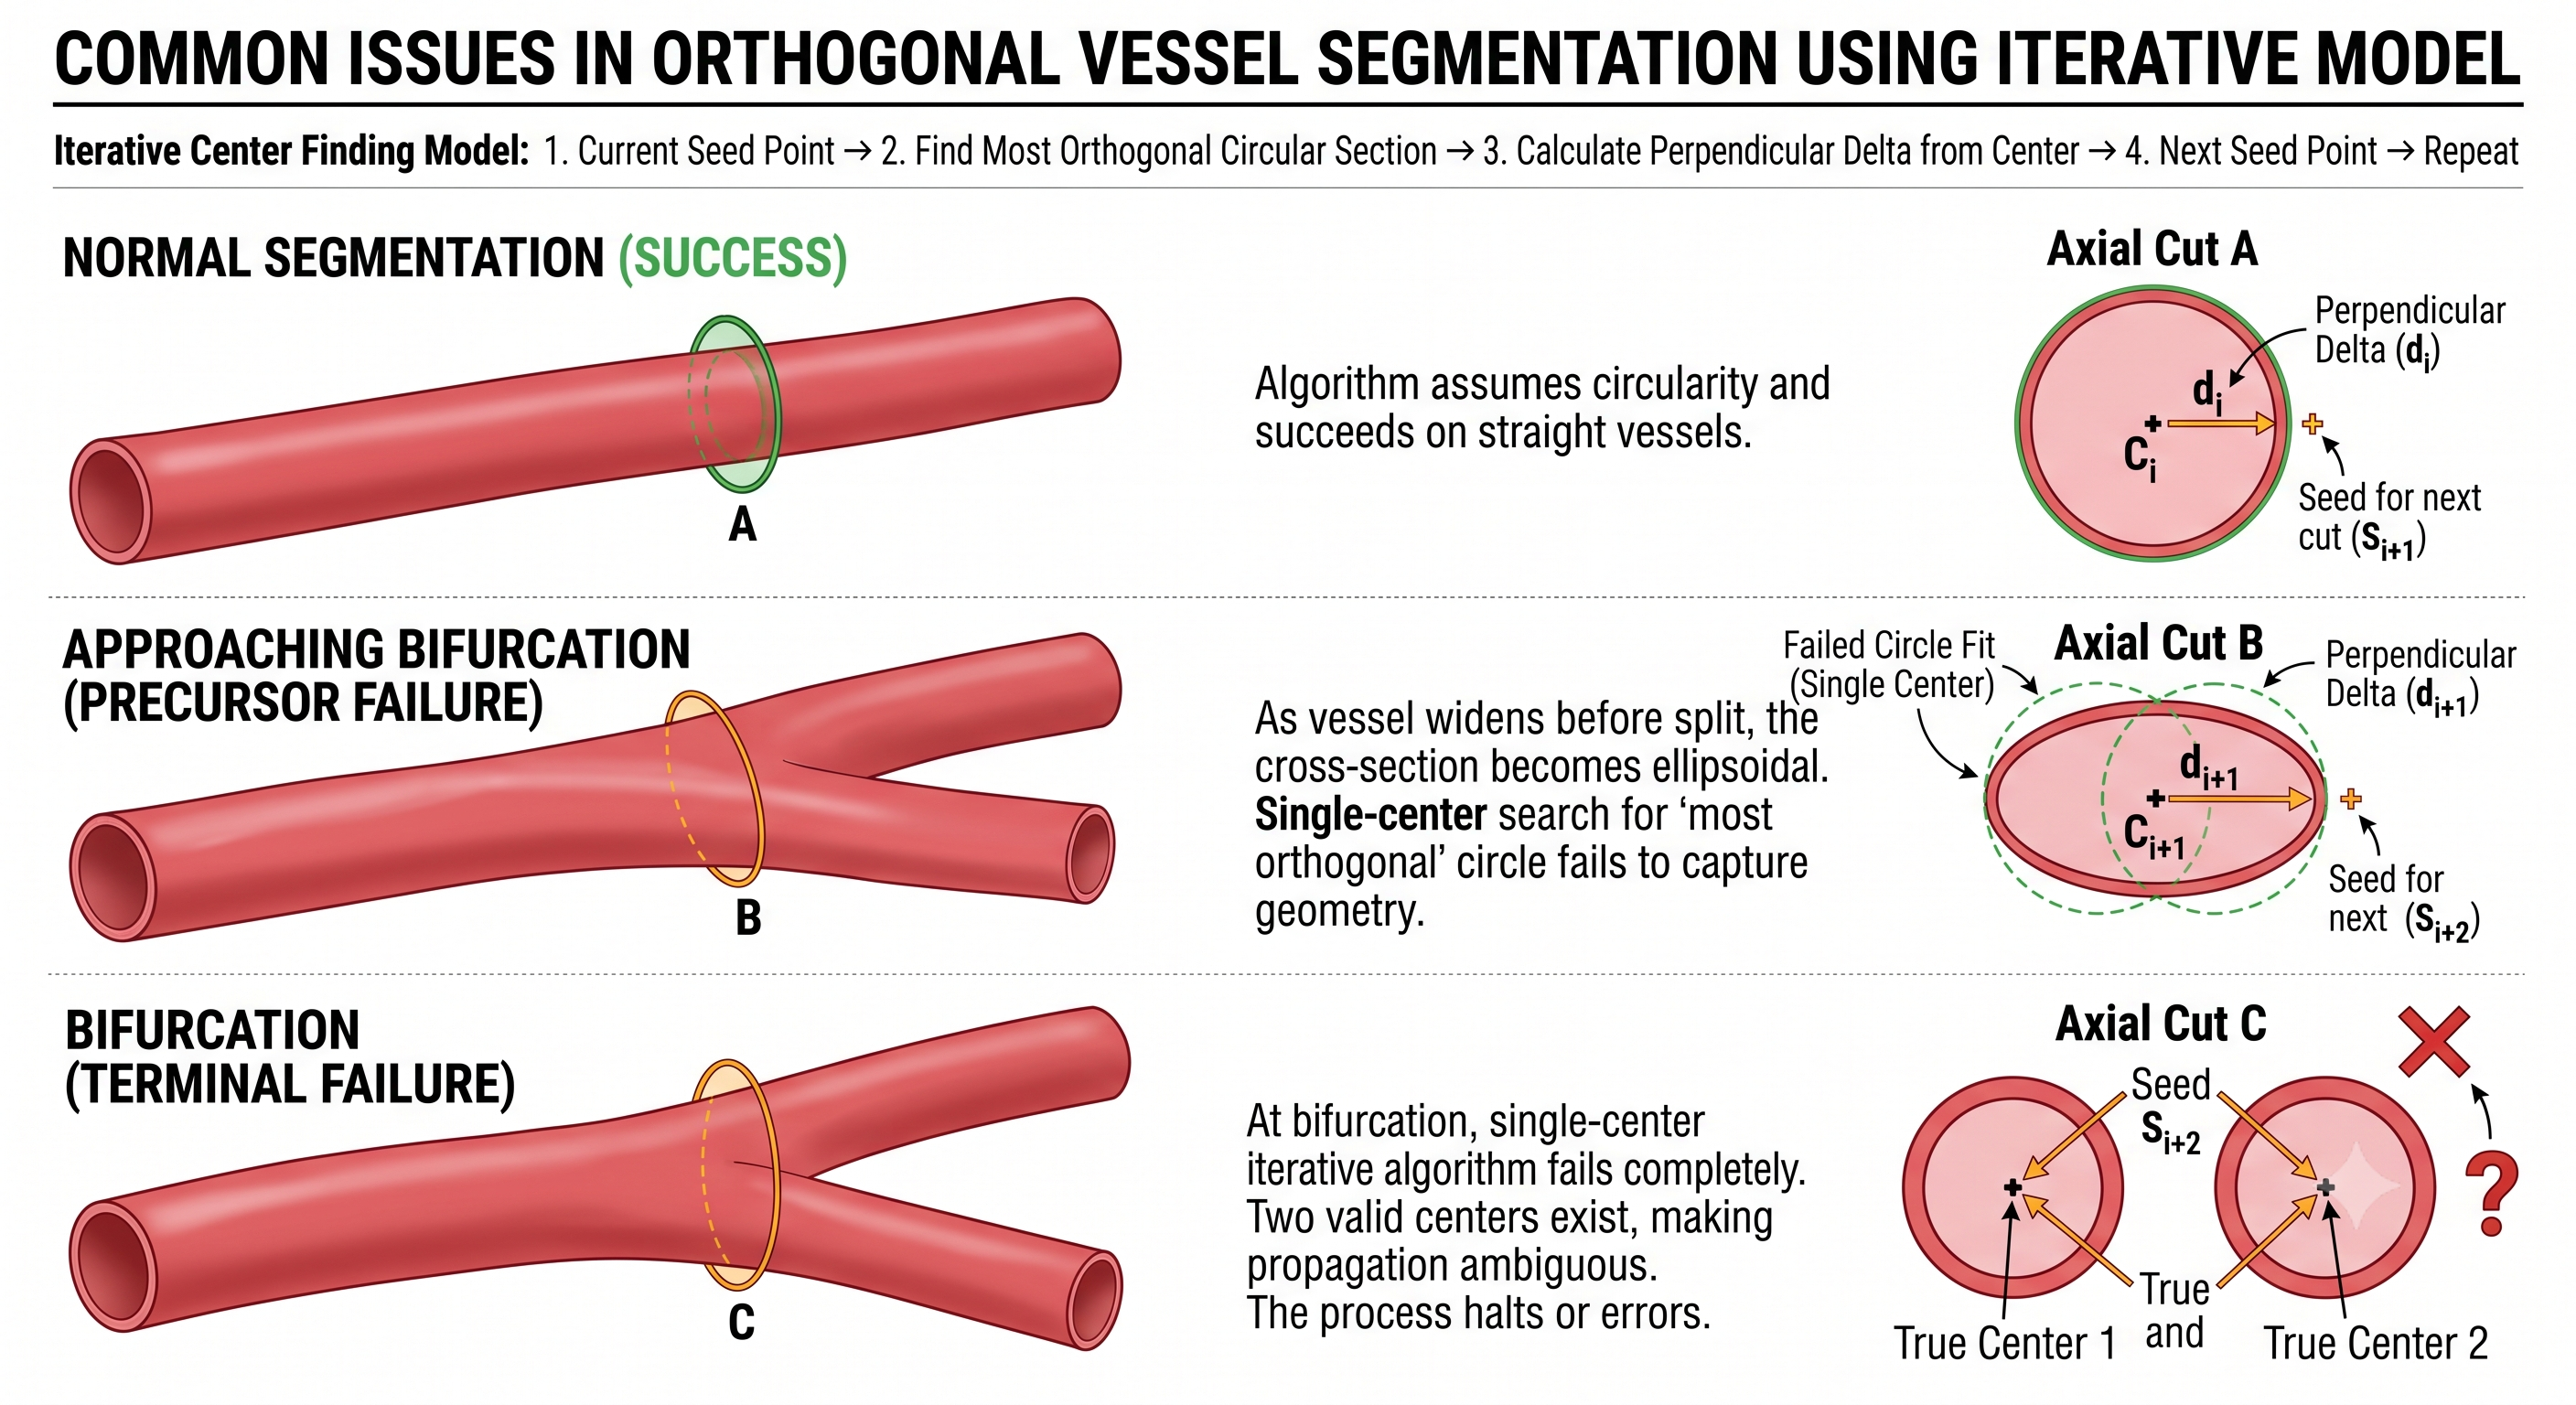
\includegraphics[width=0.85\linewidth,height=0.78\textheight,keepaspectratio]{figures/ellipse.png}
\end{frame}

\begin{frame}{IFT operational limits}
\footnotesize
\begin{columns}[T]
\begin{column}{0.48\linewidth}
\begin{block}{Hand-crafted costs}
\scriptsize
Edge weights are designed per organ and per contrast phase. Every new acquisition protocol requires re-tuning, making large-scale generalization impractical.
\end{block}
\vspace{0.1cm}
\begin{block}{Partial-volume sensitivity}
\scriptsize
At thin-walled structures (renal papillae, vessel walls, bile duct), the integer-valued boundary metric leaks through sub-voxel transitions.
\end{block}
\end{column}
\begin{column}{0.48\linewidth}
\begin{block}{Multi-class scaling}
\scriptsize
Concurrent labelling of 7+ anatomical classes (liver, kidney, pancreas, spleen, vasculature) requires sequential or competitive seeding strategies that scale poorly in time and memory.
\end{block}
\vspace{0.05cm}
\begin{alertblock}{Implication for the differentiable hybrid method}
\scriptsize
These three limits motivate the differentiable formulation: \alert{learn the costs end-to-end} while preserving the algorithmic pipeline surgeons depend on.
\end{alertblock}
\end{column}
\end{columns}
\vspace{0.1cm}
\end{frame}

\begin{frame}{Deep learning: what the literature shows}
\footnotesize
\begin{columns}[T]
\begin{column}{0.48\linewidth}
\begin{block}{Convolutional dominance}
\scriptsize
Systematic review of 52 studies (2015--2026): \textbf{98.1\,\%} use CNNs; \textbf{82.7\,\%} are 3D U-Net variants. Parenchymal organ Dice has saturated near \textbf{82\,\%}.
\end{block}
\vspace{0.1cm}
\begin{block}{Self-configuring CNNs}
\scriptsize
nnU-Net achieves \textbf{Dice $\approx$ 82.3\,\%} on BTCV with \emph{zero} task-specific tuning by inferring architecture from dataset fingerprints.
\end{block}
\end{column}
\begin{column}{0.48\linewidth}
\begin{block}{Transformer hybrids}
\scriptsize
UNETR and Swin UNETR reach \textbf{Dice $\approx$ 82.4\,\%} on BTCV -- statistically indistinguishable from nnU-Net. Architectural ceiling, not representational gap.
\end{block}
\vspace{0.15cm}
\begin{alertblock}{Vascular gap remains}
\scriptsize
Renal and portal vessels: \textbf{65--75\,\%} Dice across all paradigms. Foundation models (TotalSegmentator, MedSAM) score <70\,\% on vasculature.
\end{alertblock}
\end{column}
\end{columns}
\end{frame}

\begin{frame}{Topology and geometry-aware learning}
\footnotesize
\begin{columns}[T]
\begin{column}{0.48\linewidth}
\begin{block}{clDice: skeleton-based loss}
\scriptsize
Augments standard Dice with soft-skeleton term. Penalizes disconnected centerlines without extra inference cost. Reduces connectivity errors by \textbf{20--40\,\%} on tubular structures. Not yet applied to 3D abdominal vessels.
\end{block}
\vspace{0.1cm}
\begin{block}{Persistent homology loss}
\scriptsize
Differentiable approximation to Wasserstein distance between persistence diagrams. Enforces correct \textbf{Betti numbers}: $\beta_0$ (connected components) and $\beta_1$ (loops). Targets missed bifurcations and spurious bridges.
\end{block}
\end{column}
\begin{column}{0.48\linewidth}
\begin{block}{Branch-aware centerline loss}
\scriptsize
Penalizes missing daughter vessels at bifurcation points. Couples to the differentiable vessel tracker, which provides explicit centerline and radius estimates.
\end{block}
\vspace{0.15cm}
\begin{alertblock}{Hypothesis: topology-aware losses}
\scriptsize
Synergy: topology-aware losses + differentiable classical pipeline = topologically correct, surgeon-editable delineations with low cognitive load.
\end{alertblock}
\end{column}
\end{columns}
\end{frame}

\begin{frame}{Differentiable classical pipelines: theory and method}
\footnotesize
\begin{columns}[T]
\begin{column}{0.48\linewidth}
\begin{block}{Softening the Seeded IFT}
\scriptsize
Hard bottleneck cost: $C^*(s,t) = \min_{\pi: s\to t} \max_{e\in\pi} w(e)$

Soft approximation: $\tilde{C}^\tau(s,t) = -\tau \log \sum_{\pi: s\to t} \exp\!\Bigl(-\tfrac{1}{\tau}\textstyle\sum_{e\in\pi} w(e)\Bigr)$

Temperature $\tau \to 0^+$ recovers $C^*(s,t)$; larger $\tau$ yields smooth gradients.
\end{block}
\vspace{0.1cm}
\begin{block}{End-to-end training}
\scriptsize
Edge weights $w(e)$ are learned by the CNN feature encoder. Back-propagation through $\tilde{C}^\tau$ trains the network to minimize topology-aware losses.
\end{block}
\end{column}
\begin{column}{0.48\linewidth}
\begin{block}{Differentiable vessel tracking}
\scriptsize
Replace argmax orientation estimate with soft-attention readout over eigenvector field. Gaussian cross-section fit becomes differentiable w.r.t. learned Hessian response.
\end{block}
\vspace{0.15cm}
\begin{alertblock}{Research Gap: Unified Differentiation}
\scriptsize
Proposed research is the first to combine end-to-end differentiation of both Seeded IFT \emph{and} orthogonal vessel tracking under topology-aware losses.
\end{alertblock}
\end{column}
\end{columns}
\end{frame}

\section{Research statement}

\begin{frame}{From gaps to thesis}
\centering
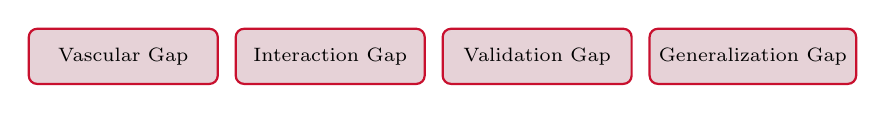
\begin{tikzpicture}[
node distance=0.2cm,
gap/.style={rectangle, draw=accent, thick, rounded corners=3pt, minimum width=2.4cm, minimum height=0.7cm, align=center, font=\scriptsize, fill=accentlight}
]
\node[gap] (g1) {Vascular Gap};
\node[gap, right=of g1] (g2) {Interaction Gap};
\node[gap, right=of g2] (g3) {Validation Gap};
\node[gap, right=of g3] (g4) {Generalization Gap};
\end{tikzpicture}

\vspace{0.4cm}
\begin{alertblock}{Thesis Statement}
  \centering\small\bfseries
  The next clinically meaningful step requires a principled fusion of the deterministic, interaction-aware pipeline with modern deep learning, evaluated on geometric AND surgeon-rated clinical utility.
\end{alertblock}
\end{frame}

\begin{frame}{Research questions}
\scriptsize
\begin{description}[leftmargin=1.0em,style=nextline]
\item[RQ1] Can a \emph{differentiable} formulation of the Seeded IFT and of orthogonal vessel tracking be trained end-to-end so as to match or exceed nnU-Net and Swin UNETR on abdominal organs while retaining the controllability and auditability of the classical algorithms?

\item[RQ2] Do topology- and geometry-aware losses (clDice, persistent homology, branch-aware centerline loss) close a measurable fraction of the 65--75\,\% Dice vascular gap and reduce Betti-number errors on abdominal vasculature?

\item[RQ3] Can foundation models (MedSAM, SAM-Med3D) be prompt-adapted to act as zero-shot priors for the hybrid framework, accelerating annotation under an active-learning protocol that compensates for the limited paired DICOM/STL legacy data at DocDo?

\item[RQ4] Does the proposed framework, exposed to surgeons through an open-source 3D editor, produce a statistically significant reduction in \emph{time-to-segmentation} and cognitive load (NASA-TLX) relative to the current DocDo deterministic pipeline, while maintaining or improving surgeon-rated segmentation quality?
\end{description}
\end{frame}

\section{Differentiable hybrid method}

\begin{frame}{The core idea}
\footnotesize
\centering
\textit{Operator-controllable algorithm, learnable costs, topology-aware objective.}
\vspace{0.15cm}
\begin{center}
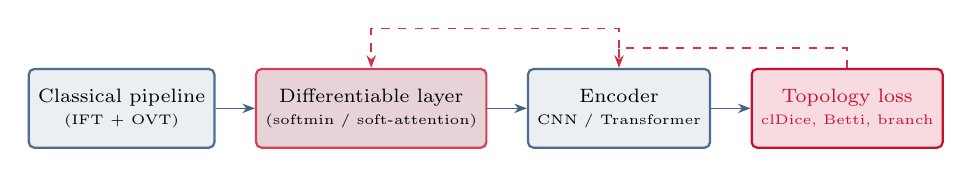
\begin{tikzpicture}[
  node distance=0.5cm,
  font=\scriptsize,
  box/.style={rectangle, draw=utadblue!70, thick, rounded corners=2pt,
              minimum width=2.3cm, minimum height=1.0cm,
              align=center, fill=utadblue!8},
  diffbox/.style={box, fill=accentlight, draw=accent!80},
  lossbox/.style={box, fill=accent!15, draw=accent, text=accent},
  fwd/.style={-{Stealth[length=1.6mm]}, semithick, utadblue!75},
  grad/.style={-{Stealth[length=1.6mm]}, semithick, accent!85, dashed}
]
  \node[box]                       (cl)  {Classical pipeline\\\tiny (IFT + OVT)};
  \node[diffbox, right=of cl]      (df)  {Differentiable layer\\\tiny (softmin / soft-attention)};
  \node[box,      right=of df]     (enc) {Encoder\\\tiny CNN / Transformer};
  \node[lossbox,  right=of enc]     (ls)  {Topology loss\\\tiny clDice, Betti, branch};

  \draw[fwd] (cl)  -- (df);
  \draw[fwd] (df)  -- (enc);
  \draw[fwd] (enc) -- (ls);

  \draw[grad] (ls.north) -- ++(0,0.25) -| (enc.north);
  \draw[grad] (enc.north) ++(0,0.25) -- ++(0,0.25) -| (df.north);
\end{tikzpicture}
\end{center}
\vspace{0.05cm}
\begin{alertblock}{Thesis}
Make IFT and OVT differentiable layers whose costs are learned end-to-end, while preserving the algorithmic pipeline surgeons depend on.
\end{alertblock}
\end{frame}

\begin{frame}{Differentiable Seeded IFT: Formulation}
\footnotesize
\begin{align*}
\textbf{Softmin Cost:} \quad & \tilde{C}^\tau(s,t) = -\tau \log \sum_{\pi:s\to t} \exp\left(-\frac{1}{\tau}\sum_{e\in\pi} w(e)\right) \\[0.25em]
\textbf{Path Probability:} \quad & p(\pi|s,t) = \frac{\exp\left(-\frac{1}{\tau}\sum_{e\in\pi} w(e)\right)}{\sum_{\pi':s\to t} \exp\left(-\frac{1}{\tau}\sum_{e'\in\pi'} w(e')\right)} \\[0.25em]
\textbf{Gradient:} \quad & \frac{\partial \tilde{C}^\tau}{\partial w(e)} = \sum_{\pi\ni e} p(\pi|s,t)
\end{align*}
\vspace{-0.1cm}
\begin{alertblock}{Theoretical Foundation (Min-Bottleneck vs.\ Sum-Path)}
\scriptsize
Hard IFT $C^* = \min_\pi \max_{e\in\pi} w(e)$ is a min-bottleneck path. The soft surrogate is a softmin of sum-path costs. They coincide only when $w(e)$ is binary; otherwise the sum form is a strict relaxation chosen for gradient flow. Deployment uses the sum form with $\tau\to0$ to yield a deterministic shortest-path forest (re-definition, not recovery).
\end{alertblock}
\end{frame}

\begin{frame}{Why this works}
\footnotesize
\vspace{0.15cm}
\begin{itemize}
\setlength\itemsep{8pt}
\item \textbf{Gradient flow:} topology-aware loss back-propagates through softmin to CNN edge-weight parameters
\item \textbf{Deterministic deployment:} at inference, harden $\tau\to 0$ to recover a deterministic shortest-path forest --- no stochasticity at test time
\item \textbf{Editability preserved:} surgeon seeds at inference time still steer the path forest --- every correction takes $\le 2$\,s
\end{itemize}
\end{frame}

\begin{frame}{Differentiable Orthogonal Vessel Tracker}
\footnotesize
Replace argmax orientation with \textbf{soft-attention readout} over eigenvector field:
\vspace{0.15cm}
\begin{itemize}
\setlength\itemsep{6pt}
\item Learnable ridge response via Hessian eigenvalue regression
\item Learnable elliptical cross-section estimator (handles non-circular vessels)
\item Differentiable step size and stopping criteria
\end{itemize}
\begin{center}
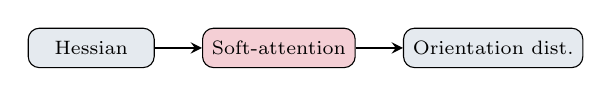
\begin{tikzpicture}[node distance=0.6cm, auto, >=stealth, font=\scriptsize]
  \node[draw, rounded corners, fill=utadblue!10, minimum width=1.6cm, minimum height=0.5cm] (hess) {Hessian};
  \node[draw, rounded corners, fill=accent!20, minimum width=1.8cm, minimum height=0.5cm, right=of hess] (attn) {Soft-attention};
  \node[draw, rounded corners, fill=utadblue!10, minimum width=2.0cm, minimum height=0.5cm, right=of attn] (orient) {Orientation dist.};
  \draw[->, thick] (hess) -- (attn);
  \draw[->, thick] (attn) -- (orient);
\end{tikzpicture}
\end{center}
\vspace{0.15cm}
{\scriptsize\color{gray} Terms: soft-attention = weighted sum over orientations (no hard argmax); orientation dist. = probability distribution over ridge directions.}
\end{frame}

\begin{frame}{Coupling with feature encoder}
\footnotesize
The end-to-end framework couples deep feature learning directly with the deterministic trackers:
\vspace{0.1cm}
\centering
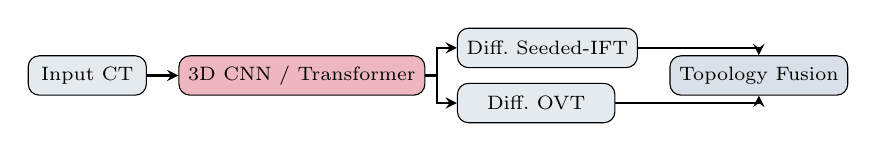
\begin{tikzpicture}[node distance=0.5cm and 0.4cm, auto, >=stealth, font=\scriptsize]
  \node[draw, rounded corners, fill=utadblue!10, minimum width=1.5cm, minimum height=0.5cm] (input) {Input CT};
  \node[draw, rounded corners, fill=accent!30, minimum width=1.8cm, minimum height=0.5cm, right=of input] (cnn) {3D CNN / Transformer};
  \node[draw, rounded corners, fill=utadblue!10, minimum width=2.0cm, minimum height=0.5cm, right=of cnn, yshift=0.35cm] (ift) {Diff.\ Seeded-IFT};
  \node[draw, rounded corners, fill=utadblue!10, minimum width=2.0cm, minimum height=0.5cm, right=of cnn, yshift=-0.35cm] (ovt) {Diff.\ OVT};
  \node[draw, rounded corners, fill=utadblue!15, minimum width=2.2cm, minimum height=0.5cm, right=of ift, yshift=-0.35cm] (fusion) {Topology Fusion};
  
  \draw[->, thick] (input) -- (cnn);
  \draw[->, thick] (cnn.east) -- +(0.15,0) |- (ift.west);
  \draw[->, thick] (cnn.east) -- +(0.15,0) |- (ovt.west);
  \draw[->, thick] (ift.east) -- +(0.15,0) -| (fusion.north);
  \draw[->, thick] (ovt.east) -- +(0.15,0) -| (fusion.south);
\end{tikzpicture}
\par
\vspace{0.15cm}
\begin{block}{Joint Training Paradigm}
\scriptsize
The 3D CNN/Transformer encoder predicts edge weights $w(e)$ and ridge responses. Gradients flow from the topology losses back through the differentiable IFT and OVT layers, updating the neural representation.
\end{block}
\end{frame}

\begin{frame}{Hypotheses}
\scriptsize
\begin{columns}[T]
\begin{column}{0.49\linewidth}
\begin{block}{H1: Seeded IFT Editability}
\scriptsize
End-to-end learning of IFT cost functions yields equal/better parenchymal Dice than nnU-Net while preserving interactive editability in $\le 2$\,s.
\end{block}
\vspace{0.1cm}
\begin{block}{H2: Vascular Topology}
\scriptsize
A topology-aware variant of the hybrid framework improves vascular Dice by $\ge 5$\,p.p.\ (percentage points) and reduces Betti-0/Betti-1 errors by $\ge 30\%$.
\end{block}
\end{column}
\begin{column}{0.49\linewidth}
\begin{block}{H3: Foundation-Model Acceleration}
\scriptsize
Prompted foundation-model priors reduce the annotation effort by $\ge 40\%$ in an active-learning loop.
\end{block}
\vspace{0.1cm}
\begin{block}{H4: Clinical Translation Utility}
\scriptsize
Surgeons using the editor are $\ge 30\%$ faster than legacy, with non-inferior quality (one-sided margin $0.5$).
\end{block}
\end{column}
\end{columns}
\end{frame}

\begin{frame}{Risks \& mitigations --- differentiable hybrid method}
\footnotesize
\vspace{0.1cm}
\begin{center}
\begin{tabular}{p{3.2cm}p{1.8cm}p{5.5cm}}
\toprule
\textbf{Risk} & \textbf{Severity} & \textbf{Mitigation} \\
\midrule
Numerical instability of soft-min & \textcolor{accent}{Medium} & Entropy regularization, gradient clipping, straight-through fallback \\
\rowcolor{accentlight}
Foundation-model contingency & \textcolor{accent}{Medium} & Restrict to parenchyma, report negative findings \\
\bottomrule
\end{tabular}
\end{center}
\end{frame}

\begin{frame}{Expected outcome --- differentiable hybrid method}
\footnotesize
\vspace{0.1cm}
\textbf{Timeline: M6--M24}
\vspace{0.1cm}
\begin{itemize}
\setlength\itemsep{6pt}
\item \textbf{M12:} Differentiable Seeded-IFT C++ prototype
\item \textbf{M18:} Differentiable OVT prototype
\item \textbf{M24:} Hybrid framework benchmarked vs.\ nnU-Net / Swin UNETR
\end{itemize}
\vspace{0.15cm}
\textbf{Deliverables:}
\begin{itemize}
\setlength\itemsep{4pt}
\item \textbf{D2.1} Open-source C++/WASM library (npm + GitHub)
\item \textbf{D2.2} Methodological paper (target: \textit{Medical Image Analysis})
\end{itemize}
\end{frame}

\section{Supporting work packages}

\begin{frame}{Foundations, data \& ethics (M1--M12)}
\footnotesize
\textbf{Tasks}
\begin{itemize}
\setlength\itemsep{0pt}
\item \textbf{T1.1} Finalize systematic review and submit for publication
\item \textbf{T1.2} Curate and harmonize public datasets into single multi-organ split
\item \textbf{T1.3} Re-voxelize retrospective DocDo STL (3D-mesh) cohort into shape-prior dataset
\item \textbf{T1.4} Prepare and submit CEP/CONEP (Brazilian ethics committees) protocol for São Marcos cohort
\item \textbf{T1.5} Specify editor data model and annotation schema
\end{itemize}
\vspace{0.1cm}
\textbf{Key deliverable:} SLR paper submission + CEP/CONEP ethics protocol for São Marcos cohort
\end{frame}

\begin{frame}{Topology-aware vascular segmentation (M18--M36)}
\centering
\vspace{0.1cm}
\fcolorbox{accent}{accentlight}{\parbox{0.88\linewidth}{\centering\textbf{clDice} --- skeleton Dice loss preserving tubular topology}}
\vspace{0.15cm}
\fcolorbox{accent}{accentlight}{\parbox{0.88\linewidth}{\centering\textbf{Persistent homology} --- Wasserstein distance on persistence diagrams}}
\vspace{0.15cm}
\fcolorbox{accent}{accentlight}{\parbox{0.88\linewidth}{\centering\textbf{Branch-aware centerline loss} --- coupled to the differentiable vessel tracker}}
\vspace{0.1cm}

\tiny Evaluation on abdominal vasculature (KiTS renal; in-house); ablations isolate each loss term
\vspace{0.1cm}

{\scriptsize\color{gray} Ablations = systematic removal of components to isolate each loss term's contribution.}
\end{frame}

\begin{frame}{Foundation-model adaptation (M24--M36)}
\footnotesize
\begin{itemize}
\setlength\itemsep{0pt}
\item \textbf{Priors:} MedSAM + SAM-Med3D prompt-tuned with clicks/scribbles from editor
\item \textbf{Zero-shot bootstrap:} foundation model as prior to accelerate annotation on São Marcos cohort
\item \textbf{Active-learning loop:} driven by predictive entropy + topology-error proxies
\item \textbf{Baselines:} direct foundation-model use (TotalSegmentator) vs.\ the differentiable hybrid and topology-aware methods alone
  \end{itemize}
\vspace{0.1cm}
\centering\fcolorbox{accent}{accentlight}{\parbox{0.7\linewidth}{\centering Target: 40\% annotation-effort reduction}}
\vspace{0.15cm}

{\scriptsize\color{gray} Terms: priors = pre-trained model weights; zero-shot = inference without task-specific training; active learning = iterative selection of informative samples; prompt-tuning = adapting model with user interactions.}
\end{frame}

\begin{frame}{Clinical validation (M30--M48)}
\footnotesize
\begin{itemize}
\setlength\itemsep{0pt}
\item \textbf{Editor:} open-source web-based 3D editor (C++/WebAssembly/WebGPU); npm + GitHub
\item \textbf{Study:} prospective surgeon study at Hospital São Marcos
\item \textbf{Sample:} $\ge 8$ surgeons, $\ge 30$ cases, pre-registered
\item \textbf{Endpoints:} time-to-segmentation, NASA-TLX (cognitive load), SUS (System Usability Scale), 5-point Likert
\item \textbf{Dataset:} anonymized São Marcos public release
  \item \textbf{Dissertation:} write and defend
  \end{itemize}
\vspace{0.1cm}
{\scriptsize\color{gray} Terms: prospective = study planned before execution; pre-registered = analysis plan preregistered; endpoints = primary outcome measures; NASA-TLX = cognitive workload questionnaire; SUS = System Usability Scale (10-item standardized usability questionnaire); Likert = 5-point agreement scale.}
\end{frame}

\begin{frame}{Schedule}
\centering
\resizebox{\textwidth}{!}{
\begin{ganttchart}[
  hgrid, vgrid,
  x unit=0.30cm, y unit chart=0.22cm,
  bar/.append style={fill=utadblue!70, draw=utadblue},
  bar incomplete/.append style={fill=utadblue!30},
  group/.append style={fill=accent!70, draw=accent},
  milestone/.append style={fill=accent!80, draw=accent},
  title/.style={draw=none, fill=none},
  title label font=\sffamily\small,
  bar label font=\sffamily\tiny,
  group label font=\sffamily\bfseries\small,
  milestone label font=\sffamily\small,
]{1}{48}
\gantttitle{Months from Oct.\,2025}{48} \\
\gantttitle{6}{6}\gantttitle{12}{6}\gantttitle{18}{6}\gantttitle{24}{6}\gantttitle{30}{6}\gantttitle{36}{6}\gantttitle{42}{6}\gantttitle{48}{6} \\
\ganttgroup{Foundations \& ethics}{1}{12} \\
\ganttbar{T1.1 Paper submission}{1}{6} \\
\ganttbar{T1.2 Public-data harmonization}{2}{9} \\
\ganttbar{T1.3 STL shape-prior dataset}{4}{10} \\
\ganttbar{T1.4 CEP/CONEP protocol}{1}{12} \\
\ganttbar{T1.5 Annotation schema}{6}{12} \\
\ganttgroup{Differentiable hybrid}{6}{24} \\
\ganttbar{T2.1 Diff.\ Seeded-IFT}{6}{15} \\
\ganttbar{T2.2 Diff.\ vessel tracker}{10}{20} \\
\ganttbar{T2.3 Backbone coupling}{14}{22} \\
\ganttbar{T2.4 Benchmarks}{18}{24} \\
\ganttmilestone{Paper submission}{24} \\
\ganttgroup{Topology-aware vessels}{18}{36} \\
\ganttbar{T3.1 clDice / PH losses}{18}{26} \\
\ganttbar{T3.2 Centerline loss}{22}{30} \\
\ganttbar{T3.3 Vascular evaluation}{26}{34} \\
\ganttbar{T3.4 Ablations}{30}{36} \\
\ganttmilestone{Paper submission}{32} \\
\ganttgroup{Foundation models}{24}{36} \\
\ganttbar{T4.1 Prompt-tuning}{24}{30} \\
\ganttbar{T4.2 Zero-shot priors}{28}{34} \\
\ganttbar{T4.3 Active learning}{30}{36} \\
\ganttbar{T4.4 Comparisons}{32}{36} \\
\ganttgroup{Validation \& thesis}{30}{48} \\
\ganttbar{T5.1 Editor v1.0 release}{30}{38} \\
\ganttbar{T5.2 Surgeon study}{36}{44} \\
\ganttbar{T5.3 Dataset release}{40}{46} \\
\ganttbar{T5.4 Dissertation}{36}{48} \\
\ganttmilestone{Defense}{48}
\end{ganttchart}
}
\end{frame}

\begin{frame}{Milestones \& go/no-go gates}
\footnotesize
\begin{description}[leftmargin=1.2em,style=nextline]
\setlength\itemsep{4pt}
\item - Ethics approved; SLR submitted; data infrastructure in place.
\item - Differentiable hybrid layer benchmarked; methodological paper submitted. \alert{\textbf{Go/no-go for topology-aware extension.}}
\item - Vascular topology paper submitted. \alert{\textbf{Go/no-go for foundation-model extension.}}
\item - Editor released; surgeon study underway.
\item - Dissertation defended.
\end{description}
\end{frame}

\begin{frame}{Risk register}
\scriptsize
\begin{center}
\begin{tabular}{p{3cm}p{2.5cm}p{2.5cm}p{4cm}}
\toprule
\textbf{Risk} & \textbf{Severity} & \textbf{Impact} & \textbf{Mitigation} \\
\midrule
\rowcolor{sevmed} Ethics delay (São Marcos) & Medium & Delays prospective cohort & Early CEP/CONEP submission; public data for early phases \\
\rowcolor{sevmed} Diff.\ IFT instability & Medium & Blocks end-to-end learning & Entropy-reg.\ softmin; straight-through fallback \\
\rowcolor{sevlow} Foundation models weak on vessels & Low & Limits O3 vascular scope & Restrict to parenchyma; report negative finding \\
\rowcolor{sevlow} Surgeon recruitment & Low & Delays clinical validation & DocDo relationship; small pre-reg.\ sample \\
\rowcolor{sevlow} Hardware bottleneck & Low & Slower training iteration & Mixed-precision; gradient accumulation; cluster scheduling \\
\rowcolor{sevmed} No scholarship / funding & Medium & Reduced candidate time & Champlain College + DocDo sustain candidate; OSS tooling \\
\rowcolor{sevlow} DocDo IP entanglement & Low & Licensing friction & Candidate holds all IP; permissive OSS licensing \\
\bottomrule
\end{tabular}
\end{center}
\end{frame}

\begin{frame}{Evaluation strategy}
\footnotesize
\begin{columns}[t]
\begin{column}{0.48\textwidth}
\begin{block}{Geometric fidelity}
\scriptsize
\begin{itemize}
\setlength\itemsep{0pt}
\item Hausdorff distances to pre-op, post-op
\item Dice, Jaccard overlap
\item Synthetic deformations with ground truth
\end{itemize}
\end{block}
\vspace{0.05cm}
\begin{block}{Topological / vascular}
\scriptsize
\begin{itemize}
\setlength\itemsep{0pt}
\item Cycle persistence (connectivity)
\item Branch counts, tree metrics
\item Per-branch volumetrics
\end{itemize}
\end{block}
\end{column}

\begin{column}{0.48\textwidth}
\begin{block}{Clinical}
\scriptsize
\begin{itemize}
\setlength\itemsep{0pt}
\item Surgeon calibration study ($n=15$)
\item Target volume errors
\item Time-to-trace
\end{itemize}
\end{block}
\vspace{0.05cm}
\begin{block}{Reliability \& robustness}
\scriptsize
\begin{itemize}
\setlength\itemsep{0pt}
\item Cross-scanner generalization
\item Pathology robustness (tumor load)
\item Inter-rater agreement
\end{itemize}
\end{block}
\end{column}
\end{columns}
\end{frame}

\section{Contributions \& closing}

\begin{frame}{Expected contributions}
\footnotesize
\begin{columns}[T]
\begin{column}{0.48\linewidth}
\textbf{Scientific}
\begin{enumerate}
\setlength\itemsep{0pt}
\item \textbf{C1} Differentiable IFT/OVT connecting classical literature to end-to-end learning
\item \textbf{C2} Vascular-gap reduction via topology-aware losses coupled to differentiable pipeline
\item \textbf{C3} Active-learning protocol using foundation models as priors under data scarcity
\item \textbf{C4} Surgeon-rated evaluation methodology complementing geometric overlap metrics
\end{enumerate}
\end{column}
\begin{column}{0.48\linewidth}
\textbf{Engineering / Clinical}
\begin{enumerate}
\setlength\itemsep{0pt}
\item \textbf{E1} Open-source web-based 3D editor (C++/WASM/WebGPU); npm + GitHub
\item \textbf{E2} Anonymized public abdominal-CT dataset from Brazilian regional hospital
\item \textbf{E3} Translation of research findings back into the DocDo clinical codebase
\end{enumerate}
\end{column}
\end{columns}
\end{frame}

\begin{frame}{Dissemination plan}
\footnotesize
\begin{itemize}
\setlength\itemsep{1pt}
\item \textbf{IEEE Access} --- systematic review (in preparation); open-source releases on GitHub, indexed on Zenodo with DOI
\item \textbf{Medical Image Analysis} --- differentiable hybrid method
\item \textbf{MICCAI} --- topology-aware vascular segmentation
\item \textbf{MIDL / MICCAI workshop} --- foundation-model adaptation
\item \textbf{IEEE Access / MedIA} --- clinical validation
\item \textbf{Scientific Data} --- dataset paper
\end{itemize}
\end{frame}

\begin{frame}{Thank you --- questions?}
\centering
\vspace{0.5cm}
{\Large \textbf{Thank you --- questions?}}
\vspace{0.4cm}

\footnotesize
Contact: \texttt{tolstenko@gmail.com} \\
Repo: \texttt{github.com/gameguild-gg/docdo-paper}
\vspace{0.3cm}


\includegraphics[height=1.2cm]{figures/utad_azul.png}
\end{frame}

\appendix

\begin{frame}{Backup --- DocDo production pipeline (legacy)}
\centering
\footnotesize
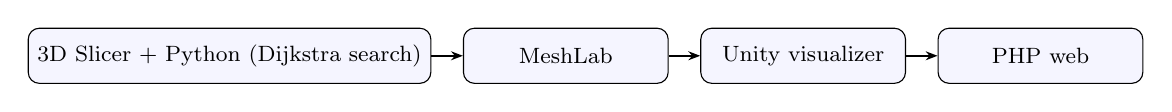
\begin{tikzpicture}[
  node distance=0.4cm,
  box/.style={rectangle, draw, rounded corners, minimum width=2.6cm, minimum height=0.7cm, align=center, font=\footnotesize, fill=blue!4},
  arr/.style={-{Stealth[length=1.5mm]}, thick}
]
  \node[box] (a) {3D Slicer + Python (Dijkstra search)};
  \node[box, right=of a] (b) {MeshLab};
  \node[box, right=of b] (c) {Unity visualizer};
  \node[box, right=of c] (d) {PHP web};
  \draw[arr] (a) -- (b);
  \draw[arr] (b) -- (c);
  \draw[arr] (c) -- (d);
\end{tikzpicture}

\vspace{0.3cm}
Operational for 1000+ cases over 10+ years
\end{frame}

\begin{frame}{Backup --- DocDo Data Pipeline \& Target Architecture}
\centering
\tiny
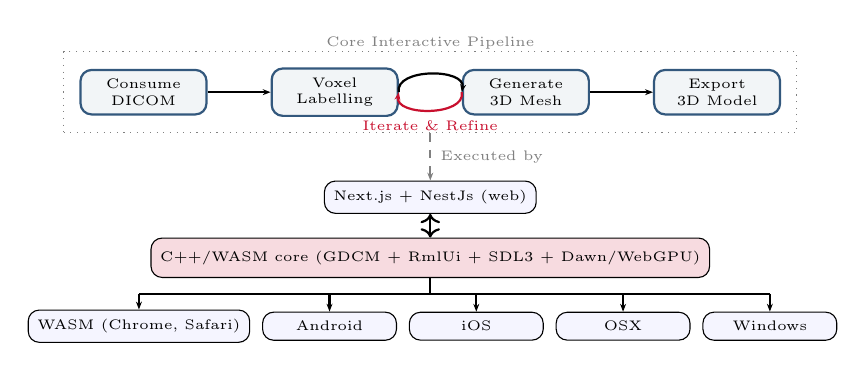
\begin{tikzpicture}[
  node distance=0.25cm and 0.4cm,
  core/.style={rectangle, draw, rounded corners, minimum width=6cm, minimum height=0.5cm, align=center, font=\tiny, fill=accent!15},
  top/.style={rectangle, draw, rounded corners, minimum width=2.5cm, minimum height=0.4cm, align=center, font=\tiny, fill=blue!4},
  tgt/.style={rectangle, draw, rounded corners, minimum width=1.7cm, minimum height=0.35cm, align=center, font=\tiny, fill=blue!4},
  pipe/.style={rectangle, draw=utadblue!80, thick, rounded corners, minimum width=1.6cm, minimum height=0.45cm, align=center, font=\tiny, fill=utadblue!5},
  arr/.style={-{Stealth[length=1mm]}, thick},
  looparr/.style={-{Stealth[length=1mm]}, thick, accent}
]

  % --- 1. DATA PIPELINE (Top) ---
  \node[pipe] (dicom) {Consume\\DICOM};
  \node[pipe, right=0.8cm of dicom] (label) {Voxel\\Labelling};
  \node[pipe, right=0.8cm of label] (mesh) {Generate\\3D Mesh};
  \node[pipe, right=0.8cm of mesh] (model) {Export\\3D Model};

  % Forward pipeline flow
  \draw[arr] (dicom) -- (label);
  \draw[arr] (label.east) to[bend left=100] (mesh.west);
  \draw[arr] (mesh) -- (model);
  
  % Iteration loop (Voxel Labelling <-> Generate Mesh)
  \draw[looparr] (mesh.west) to[bend left=100] node[below, font=\tiny, text=accent] {Iterate \& Refine} (label.east);

  % Dotted box to group the pipeline
  \node[draw=gray, dotted, inner sep=0.2cm, fit=(dicom) (label) (mesh) (model), label={[font=\tiny, gray, yshift=-0.1cm]above:Core Interactive Pipeline}] (pipebox) {};

  % --- 2. TARGET ARCHITECTURE (Bottom) ---
  \node[top, below=0.6cm of pipebox] (web) {Next.js + NestJs (web)};
  \node[core, below=0.3cm of web] (c) {C++/WASM core (GDCM + RmlUi + SDL3 + Dawn/WebGPU)};
  
  \node[tgt, below=0.4cm of c, xshift=-3.7cm] (wasm) {WASM (Chrome, Safari)};
  \node[tgt, right=0.15cm of wasm] (and) {Android};
  \node[tgt, right=0.15cm of and] (ios) {iOS};
  \node[tgt, right=0.15cm of ios] (osx) {OSX};
  \node[tgt, right=0.15cm of osx] (win) {Windows};
  
  % Connect Pipeline box to Architecture
  \draw[arr, dashed, gray] (pipebox.south) -- node[right, font=\tiny] {Executed by} (web.north);

  % Connections for architecture
  \draw[arr, <->] (web) -- (c);
  \coordinate (bus) at ($(c.south)+(0,-0.2)$);
  \draw[thick] (c.south) -- (bus);
  \draw[thick] (bus -| wasm.north) -- (bus -| win.north);
  
  \draw[arr] (bus -| wasm.north) -- (wasm.north);
  \draw[arr] (bus -| and.north) -- (and.north);
  \draw[arr] (bus -| ios.north) -- (ios.north);
  \draw[arr] (bus -| osx.north) -- (osx.north);
  \draw[arr] (bus -| win.north) -- (win.north);

\end{tikzpicture}
\end{frame}

\begin{frame}{Backup --- Webpage screenshot}
\centering

\includegraphics[height=0.65\textheight]{figures/docdo-webpage.png}

\vspace{0.15cm}
\footnotesize Next.js web with login/register, upload, HIPAA-compliant DAC.
\end{frame}

\begin{frame}{Backup --- SLR methodology + datasets}
\scriptsize
\begin{columns}[T]
\begin{column}{0.48\linewidth}
\textbf{PRISMA flow}
\begin{itemize}\itemsep1pt
  \item 2821 records (PubMed, arXiv, Semantic Scholar)
  \item 638 ES pre-filter (strict IC1--IC5 Boolean)
  \item 161 AI screening (GPT multi-model)
  \item 63 full-text assessed
  \item 52 included in synthesis
\end{itemize}
\vspace{0.15cm}
Inter-rater $\kappa = 0.89$ (10\% stratified audit)
\end{column}
\begin{column}{0.50\linewidth}
\textbf{Datasets}\\[2pt]
\tiny
\begin{tabular}{p{2.1cm}p{1.8cm}p{1.8cm}}
\textbf{Dataset} & \textbf{Size} & \textbf{Coverage} \\
KiTS21 & 489 vol & kidney + tumour \\
BTCV & 50 vol & 13 organs \\
AMOS & 500 CT + 100 MRI & 15 organs \\
MSD & 2633 total / 10 tasks & multi-organ \\
TotalSegmentator & 1228 vol & 117 structures \\
S\~ao Marcos (prospective) & cohort TBD & abdominal CT \\
\end{tabular}
\end{column}
\end{columns}
\end{frame}

\end{document}